\documentclass[conference]{IEEEtran}
\IEEEoverridecommandlockouts
% The preceding line is only needed to identify funding in the first footnote. If that is unneeded, please comment it out.
\usepackage{cite}
\usepackage{amsmath,amssymb,amsfonts}
\usepackage{algorithmic}
\usepackage{graphicx}
\usepackage{textcomp}
\usepackage{caption}
\usepackage[bosnian]{babel}

\usepackage{subcaption}
\usepackage{dblfloatfix}
\usepackage{tablefootnote}
\usepackage{xcolor}
\usepackage[T1]{fontenc}
\usepackage{etoolbox}
\usepackage{hyperref}
\hypersetup{
    colorlinks=true,
    linkcolor=blue,
    filecolor=magenta,      
    urlcolor=cyan,
}

\urlstyle{same}
\patchcmd{\thebibliography}{\section*{\refname}}{}{}{}
\def\BibTeX{{\rm B\kern-.05em{\sc i\kern-.025em b}\kern-.08em
    T\kern-.1667em\lower.7ex\hbox{E}\kern-.125emX}}
\begin{document}

\title{Klasifikacija produkata na self-checkout kasi\\}

\author{\IEEEauthorblockN{Adisa Bolić}
\IEEEauthorblockA{\textit{Prirodno-matematički fakultet} \\
\textit{Univerzitet u Sarajevu}\\
Sarajevo, Bosna i Hercegovina\\
adisa.bolic@gmail.com}
}

\maketitle

\begin{abstract}
Doskoro većina self-checkout kasa u prodavnicama je radila na principu da kupac pomoću skenera skenira barkodove svih produkata i na taj način izvrši kupovinu. Današnja revolucija u polju mašinskog učenja omogućava da se ovaj proces ubrza na način da korisnik samo postavi sve produkte na neku površinu (iznad koje se nalazi kamera) i da se potom automatski detektuje koji se proizvodi tu nalaze. Ovaj rad ima za cilj izvršenje dijela ovog procesa, tj. klasifikaciju produkata koristeći konvolucijsku neuralnu mrežu. Kod je dostupan na \href{https://github.com/adisabolic/product_classification}{GitHub repositoriju}. Za implementaciju korišten je jezik Python te biblioteka PyTorch za sve elemente mašinskog učenja.
\end{abstract}

\begin{IEEEkeywords}
self-checkout, convolutional neural network, classification, machine learning
\end{IEEEkeywords}

\section{Uvod}
Kako bi se ubrzao i pojednostavio proces kupovine u supermarketima ili restoranima u ovom radu će biti prikazan algoritam koji vrši klasifikaciju produkata na osnovu njihovih slika. Za algoritam je korištena konvolucijska neuralna mreža ResNet50 (detaljnije o arhitekturi ove mreže na \cite{b1}) koja je pretrenirana na ImageNet skupu podataka. ImageNet \cite{b2} je označen skup slika sa približno $20,000$ kategorija sa nekoliko stotina slika u svakoj kategoriji. Na slici \ref{fig1} prikazano je nekoliko slika iz ovog skupa. ILSVRC \cite{b3} (ImageNet Large Scale Visual Recognition Challenge) je takmičenje koje se godišnje održavalo u kojem je bio cilj napraviti model koji će imati što veću preciznost na ovom skupu slika. Ovo takmičenje predstavlja standard za procjenu koliko je neki model dobar. Pored toga, modeli koji su pretrenirani na ImageNet skupu se koriste (u smislu da se kopiraju težine naučene u toj pretreniranoj mreži) kada se želi trenirati model za neki drugi problem, pri čemu se izvrše određene izmjene na mreži (uglavnom se promijene dimenzije zadnjeg sloja mreže da bi odgovaralo broju kategorija u problemu koji se rješava).

\begin{figure}[htbp]
\centerline{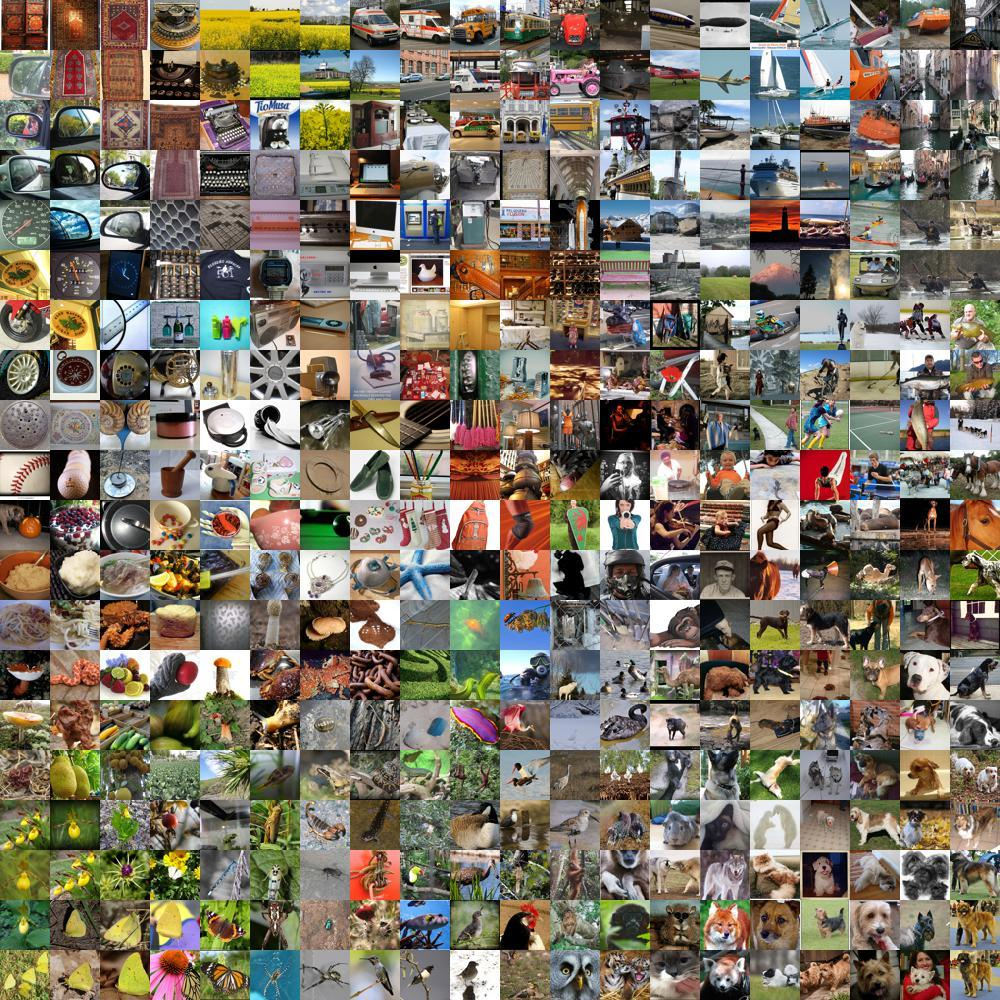
\includegraphics[width=\columnwidth]{fig1.jpg}}
\caption{Primjer slika iz ImageNet skupa slika. \href{https://cs.stanford.edu/people/karpathy/cnnembed/}{Izvor slike}}
\label{fig1}
\end{figure}
\\

U radu \cite{b4} navedeno je da se konvolucijske neuralne mreže mogu opisati kao nadogradnja nad običnim višeslojnim unaprijednim mrežama. Konvolucijska, kao i obična neuralna mreža sastoji se od jednog ulaznog, jednog izlaznog i jednog ili više skrivenih slojeva. Kod konvolucijskih neuralnih mreža specifični su konvolucijski slojevi i slojevi sažimanja.
Osim njih često se koriste i potpuno povezani slojevi. Konvolucijske neuronske mreže najčešće kreću s jednim ili više konvolucijskih slojeva, zatim slijedi sloj sažimanja, pa ponovo konvolucijski sloj i tako nekoliko puta. Mreža najčešće završava s jednim ili više potpuno povezanih slojeva koji služe za klasifikaciju. Arhitektura konvolucijskih neuronskih mreža pokazala se izrazito dobra u radu sa slikama i prepoznavanju objekata od interesa sa istih. Na slici \ref{fig2} prikazana je arhitektura jedne od prvih konvolucijskih neuralnih mreža poznate pod imenom LeNet \cite{b5}. Danas postoje mnoge modifikacije ovih mreža koje su se pokazale jako uspješne za razne probleme klasifikacije i detekcije objekata. Detaljnije o ovim mrežama kao i ostalim poljima mašinskog učenja koji su doveli do kreiranja konvolucijskih mreža može se pročitati u radu \cite{b6}. 

\begin{figure}[htbp]
\centerline{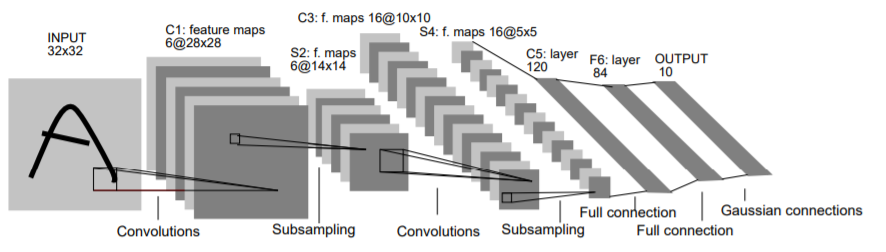
\includegraphics[width=\columnwidth]{fig2.png}}
\caption{Arhitektura LeNet \cite{b5} konvolucijske neuralne mreže. Izvor slike \cite{b5}}
\label{fig2}
\end{figure}
\\

U problemu koji se rješava u ovom radu dat je skup od približno $45,000$ slika sa ukupno $76$ klasa produkata. Slike su podijeljenje na tri dijela: trening, validacijski i testni skup. Trening i validacijski skup se koriste za treniranje (validacijski skup se koristi za smanjenje brzine učenja ukoliko se preciznost smanji nakon neke epohe sa ciljem izbjegavanja overfitinga na trening skupu, kao i za odabir najboljeg modela), dok se testni skup koristi nakon treniranja za provjeru preciznosti modela. Primjer tri slike iz skupa dat je na slici \ref{fig3}.

\begin{figure}[htbp]
\centerline{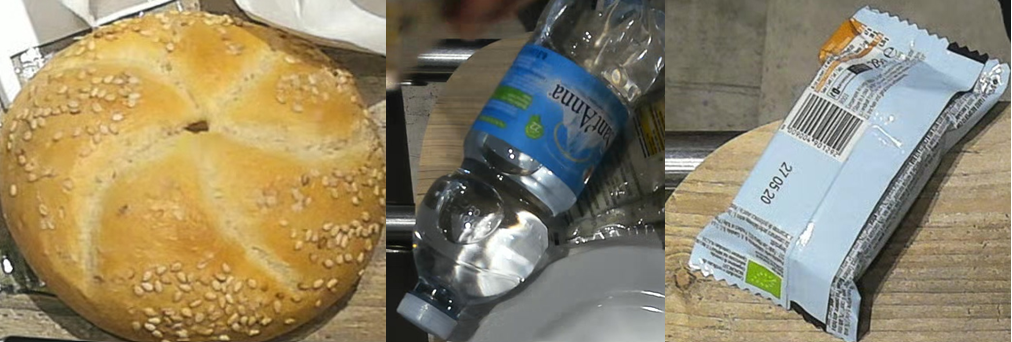
\includegraphics[width=\columnwidth]{fig3.png}}
\caption{Primjer tri slike iz trening skupa slika. Klase ovih slika su, redom, kiflica, flaširana voda i čokoladica.}
\label{fig3}
\end{figure}
\\

\section{Pregled Literature}

Proces kupovine u supermarketima se može i dodatno ubrzati. Poznat primjer ovog ubrzanja prisutan je Amazonovim Go prodavnicama, gdje kupci samo pokupe artikle koje žele sa polica i izađu iz prodavnice, a preko aplikacije im se automatski obračuna cijena kupovine. U prodavnici je prisutan veliki broj kamera koje prate sve što kupac radi i pomoću algoritma mašinskog učenja se detektuje kada kupac nešto uzme sa police sa ciljem da to nešto i kupi. Znatno je teže dizajnirati model za ovaj problem zbog mnogobrojnih situacija koje mogu nastati. Detalje i poteškoće kod ovog problema mogu se pročitati u radu \cite{b7}. 

\section{Opis modela}

Kao što je ranije spomenuto, korištena je pretrenirana ResNet50 arhitektura konvolucijske mreže. Bitni parematri kod treniranja su:

\begin{itemize}
  \item batch veličina = 128
  \item broja epoha = 20
  \item broj klasa = 76
  \item veličina trening skupa = 33,991
  \item veličina validacijskog skupa = 8456
  \item veličina testnog skupa = 2200
  \item korištene transformacije i augmentacije: normalizacija, horizonatlni i vertikalni flip, rotacija
  \item dimenzije slika: $224\times224$
  \item loss funkcija: Cross-entropy loss
\end{itemize}

Trenirana su dva modela. U prvom modelu su trenirani svi parametri mreže, dok su u drugom modelu trenirane samo težine u zadnjem fully-connected sloju mreže. Oba modela trenirana su sa istim hiperparametrima. Trening je na tri Nvidia GeForce GTX 1080 grafičke trajao oko $30$ i $17$ minuta, redom. Pošto su sve slike sa dobrim osvjetljenjem i dobre kvalitete, za očekivati je da će mreža vršiti dobre predikcije. Prvi model bi trebao davati bolje rezultate, jer se trenira čitava mreža, a ne samo zadnji sloj. 

Na slici \ref{fig4} dato je nekoliko primjera slika iz skupa nakon primijenjih transformacija.  

\begin{figure}[htbp]
\centerline{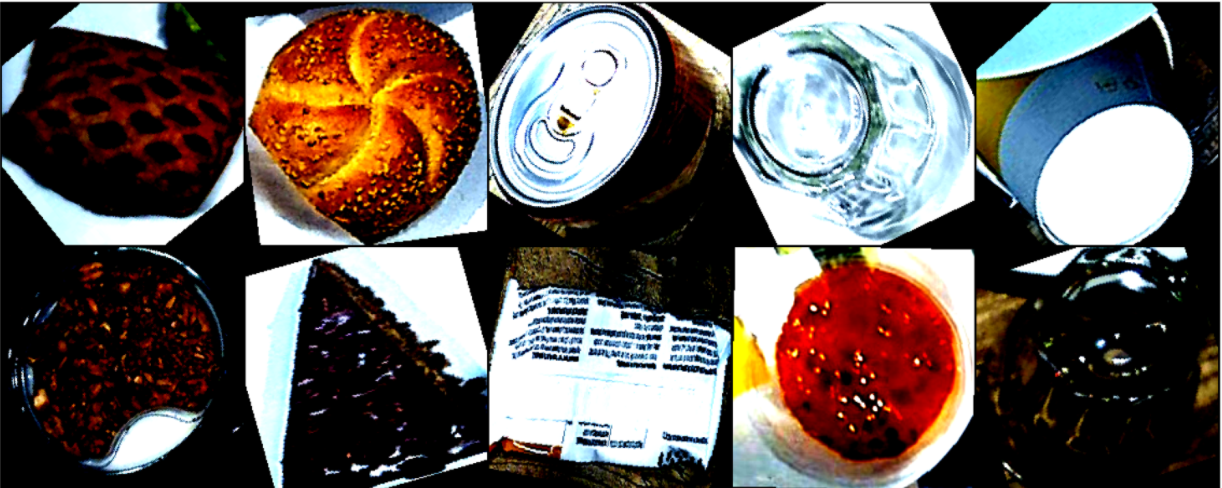
\includegraphics[width=\columnwidth]{fig4.png}}
\caption{Primjer nekoliko slika iz trening skupa nakon primijenjenih transformacija. Boja slika se promijenila uslijed normalizacije.}
\label{fig4}
\end{figure}
\\

\section{Rezultati}

Na slici \ref{fig5} prikazani su rezultati tokom treniranja prvog modela u prvih i zadnjih nekoliko epoha. Slično, na slici \ref{fig6} prikazani su rezultati tokom treniranja drugog modela. Treba primijetiti kako je pretpostavka da će prvi model davati bolje rezultate tačna. Međutim, potrebno je provjeriti preciznost oba modela na testnom skupu, pošto je moglo doći do overfitanja na trening skupu. Rezultati na testnom skupu oba modela dati su na slici \ref{fig7}. 

\begin{figure}[htbp]
\centerline{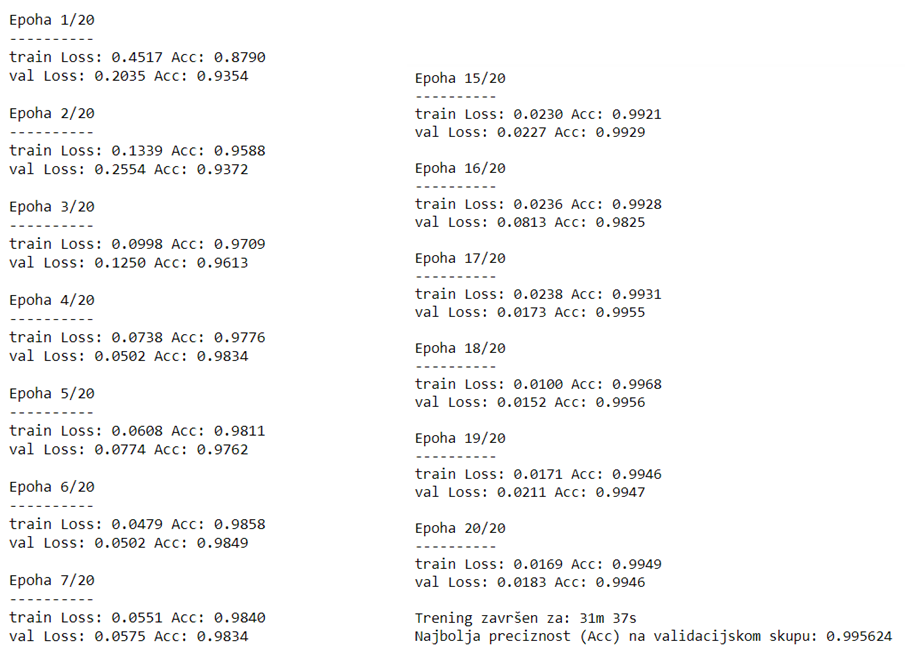
\includegraphics[width=\columnwidth]{fig5.png}}
\caption{Preciznost i vrijednost loss funkcije (na trening i validacijskom skupu) prvog modela (u kojem se svi parametri mreže treniraju) tokom prvih i zadnjih par epoha.}
\label{fig5}
\end{figure}
\\

\begin{figure}[htbp]
\centerline{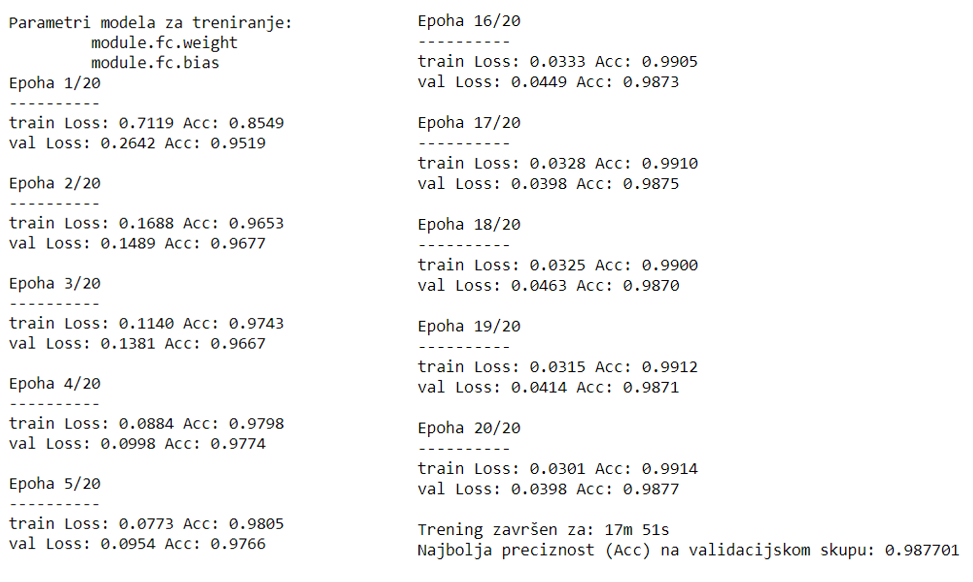
\includegraphics[width=\columnwidth]{fig6.png}}
\caption{Preciznost i vrijednost loss funkcije (na trening i validacijskom skupu) drugog modela (u kojem se samo parametri zadnjeg sloja mreže treniraju) tokom prvih i zadnjih par epoha.}
\label{fig6}
\end{figure}
\\

Pošto su rezultati na testnom skupu slični rezultatima tokom treniranja, znači da nije došlo do overfitanja i model radi ispravno sa velikom preciznošću. Mnogo više detalja i vizualizacija dostupno je u Jupyter Notebooku sa implementiranim kodom na \href{https://github.com/adisabolic/product_classification}{GitHub respositoriju}.

\begin{figure}[htbp]
\centerline{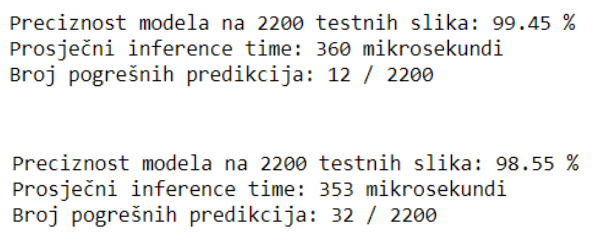
\includegraphics[width=\columnwidth]{fig7.png}}
\caption{Preciznost prvog (gore) i drugog (dole) modela na testnom skupu slika. Inference time predstavlja vrijeme koje je potrebno modelu za klasifikaciju jedne slike.}
\label{fig7}
\end{figure}
\\

\section{Zaključak}

U ovom radu kreiran je model konvolucijske neuralne mreže za klasifikaciju produkata u restoranu na ukupno $76$ klasa. Korištena je pretrenirana (na ImageNet \cite{b2} skupu slika) ResNet50 \cite{b1} mreža. Postignuta je velika preciznost mreže od $99.45\%$ na testnom skupu slika. U budućnosti je planirano napraviti model koji će vršiti detekciju objekata (da iz slike cijele scene detektuje sve produkte, lokalizira ih i potom klasificira). 


\section{Reference}
\begin{thebibliography}{00}
\bibitem{b1} Kaiming He, Xiangyu Zhang, Shaoqing Ren, Jian Sun, Deep Residual Learning for Image Recognition, 2015
\bibitem{b2} ImageNet skup slika https://www.image-net.org/about.php
\bibitem{b3} Olga Russakovsky*, Jia Deng*, Hao Su, Jonathan Krause, Sanjeev Satheesh, Sean Ma, Zhiheng Huang, Andrej Karpathy, Aditya Khosla, Michael Bernstein, Alexander C. Berg and Li Fei-Fei. (* = equal contribution) ImageNet Large Scale Visual Recognition Challenge. IJCV, 2015
\bibitem{b4} Damir Kopljar, Konvolucijske neuronske mreže, Sveučilište u Zagrebu, Fakultet elektrotehnike i računarstva, 2016 
\bibitem{b5} Yann LeCun, Leon Bottou, Yoshua Bengio, Patrick Haffner, Gradient-Based Learning Applied to Document Recognition, 1988
\bibitem{b6} Ian Goodfellow, Yoshua Bengio, Aaron Courville, Deep Learning, MIT Press, 2016
\bibitem{b7} Kirti Wankhede, Bharati Wukkadada, Vidhya Nadar, Just Walk-Out Technology and its Challenges: A Case of Amazon Go, IEEE, 2018

\end{thebibliography}
\end{document}
